\documentclass{beamer}

\usepackage{tikz}
\usepackage{pgfplots}

\setbeamertemplate{footline}[frame number]
\title{High Availability For Key-Value Stores Using Checkpoint/Restore}
\author{Fadhil Abubaker, Hussain Sadiq Abuwala}
\date{}

\begin{document}

\frame{\titlepage}

\begin{frame}
  \frametitle{Introduction}

  \begin{itemize}
    \item Modern distributed systems are expected to be highly available. \pause
  \end{itemize}

  \begin{itemize}
    \item High-availability is implemented through replication.
    \begin{itemize}
      \item Synchronous vs Asynchronous.
      \item Active-Active vs Active-Standby. \pause
    \end{itemize}
  \end{itemize}

  \begin{itemize}
    \item But implementing HA is difficult.
    \begin{itemize}
      \item Propagate updates.
      \item Coordinate transactions.
      \item Atomic handover.
      \item Performance. \pause
    \end{itemize}
  \end{itemize}

  \begin{itemize}
    \item Rely on an external layer to provide replication?
  \end{itemize}
\end{frame}

\begin{frame}{External Replication Layer}

  Push replication outside of the database system, delegating it to an external
  layer.

  \begin{itemize}
    \pause \item Shared-Disk
    \pause \item SHADOW\footnotemark
    \pause \item Distributed Replicated Block Device (DRBD)
    \pause \item Virtual Machine Replication
    \pause \item ...Checkpoint/Restore?
  \end{itemize}

  \footnotetext[1]{J. Kim, K. Salem, K. Daudjee, A. Aboulnaga, and X. Pan. Database High
  Availability Using SHADOW Systems.}
\end{frame}

\begin{frame}{Checkpoint/Restore In Userspace (CRIU)}
  \begin{itemize}
    \item Linux utility to checkpoint/restore in-memory state of a process/container. \pause
    \item A running application can be checkpointed to persistent storage as a set of files. \pause
    \item The application can be then restored back to the point it was frozen
    using the checkpoint files. \pause
    \item Integrated with container runtimes such as OpenVZ, LXC/LXD, Docker, Podman, etc.
    \item Commonly used for container live-migration.
  \end{itemize}
\end{frame}

\begin{frame}{System Architecture}
  \framesubtitle{Normal Operation}

  \begin{columns}
    \column{0.4\textwidth}
    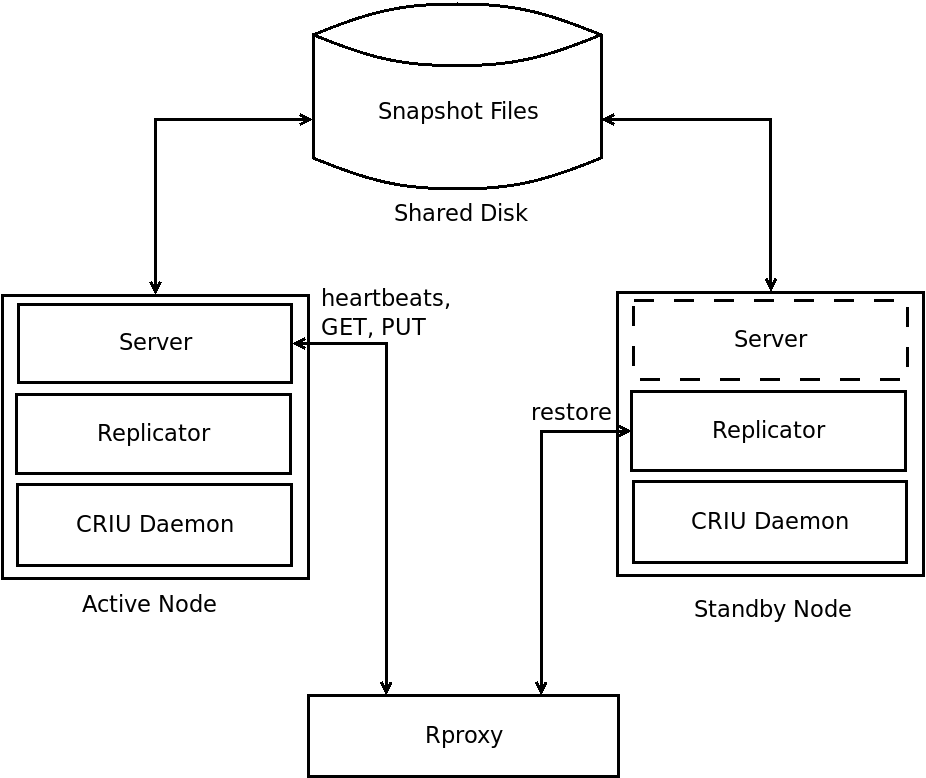
\includegraphics[scale=0.15]{../paper/arch}

    \column{0.6\textwidth}
    \begin{itemize}
      \pause \item clients send requests to the \textbf{rproxy}.
      \pause \item request is forwarded to the active \textbf{server}.
      \pause \item \textbf{server} calls \texttt{checkpoint} endpoint on the \textbf{replicator} after $n$ updates.
      \pause \item \textbf{replicator} interfaces with the \textbf{C/R daemon} and saves a snapshot to the shared-disk.
    \end{itemize}
  \end{columns}
\end{frame}

\begin{frame}{System Architecture}
  \framesubtitle{Failover Process}

  \begin{columns}
    \column{0.4\textwidth}
    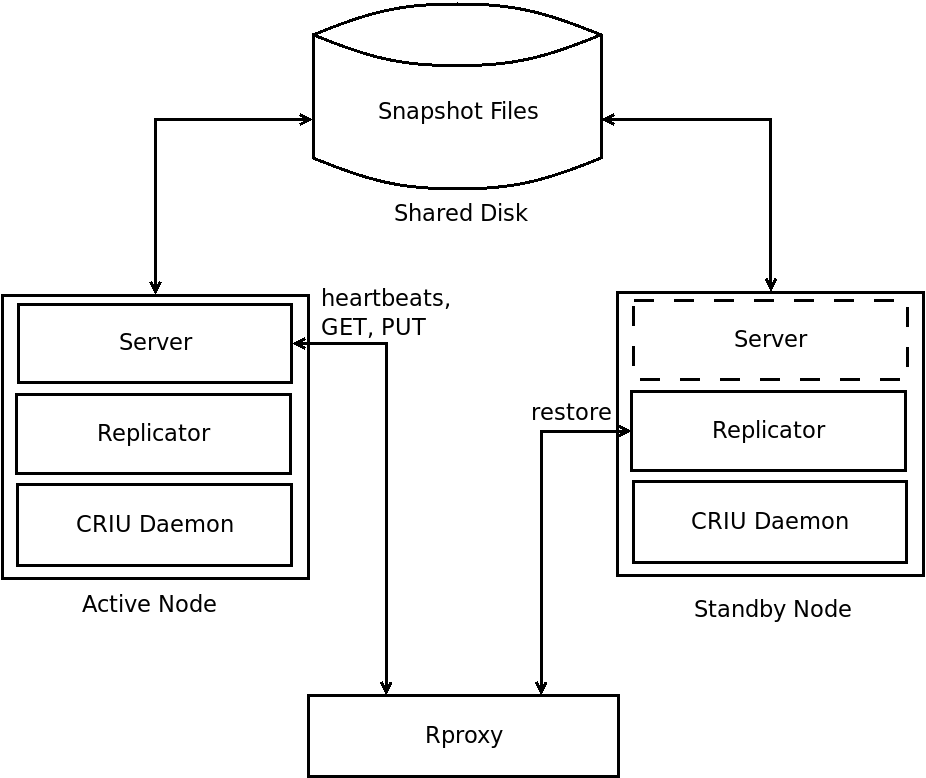
\includegraphics[scale=0.15]{../paper/arch}

    \column{0.6\textwidth}
    \begin{itemize}
      \item \textbf{rproxy} sends regular heartbeats to active \textbf{server}.
      \pause \item On timeout, calls the \texttt{restore} endpoint on standby \textbf{replicator}.
      \pause \item \textbf{replicator} restores the \textbf{server} from the latest snapshot on the shared-disk.
      \pause \item Normal operations resume, with requests forwarded to the standby.
    \end{itemize}
  \end{columns}
\end{frame}

\begin{frame}{Evaluation}
  \framesubtitle{Methodology}

  \begin{itemize}
    \item Yahoo! Cloud Serving Benchmark.
    \item Implemented a custom YCSB interface to support our key-value store.
    \item Each workload consists of 1000 operations.
    \item Workload A: 50/50 read/write mix.
    \item Workload B: 95/5 read/write mix.
    \item Snapshots were captured after every 250 updates.
  \end{itemize}
\end{frame}

\begin{frame}{Evaluation}
  \framesubtitle{Storage Performance vs Redis (No Replication)}

  \begin{columns}
    \column{0.5\textwidth}
    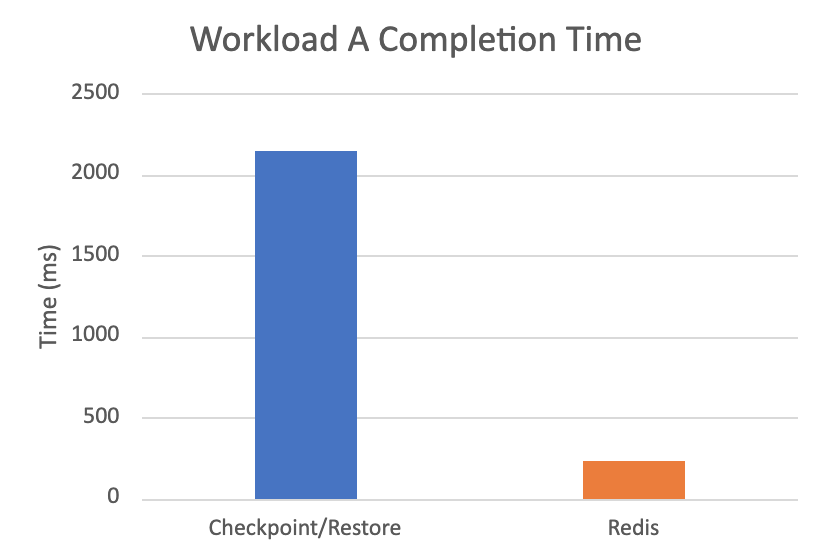
\includegraphics[scale=0.4]{../paper/redis-workload-A}

    \column{0.5\textwidth}
    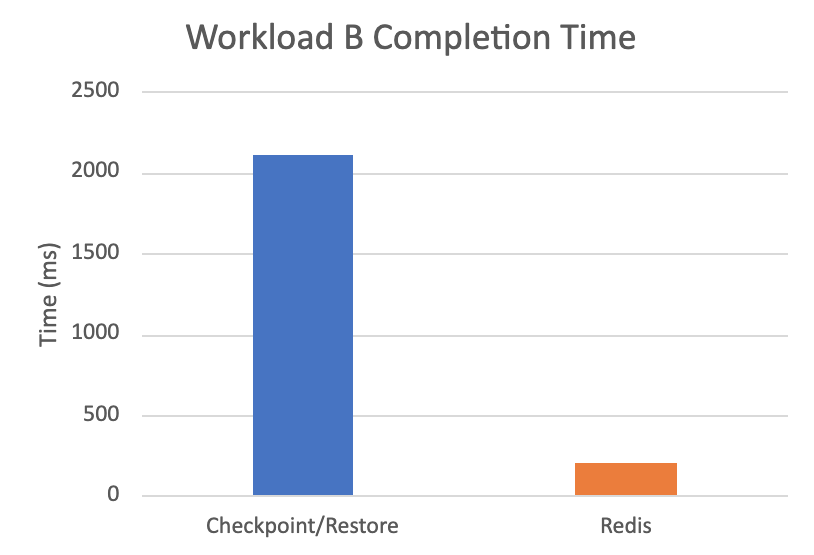
\includegraphics[scale=0.2]{../paper/redis-workload-B}
  \end{columns}

  \hspace{1cm}

  \centering
  Storage performance likely suffers due to HTTP and JSON overhead.
\end{frame}

\begin{frame}{Evaluation}
  \framesubtitle{Replication Performance vs Asynchronous Replication}

  \centering
  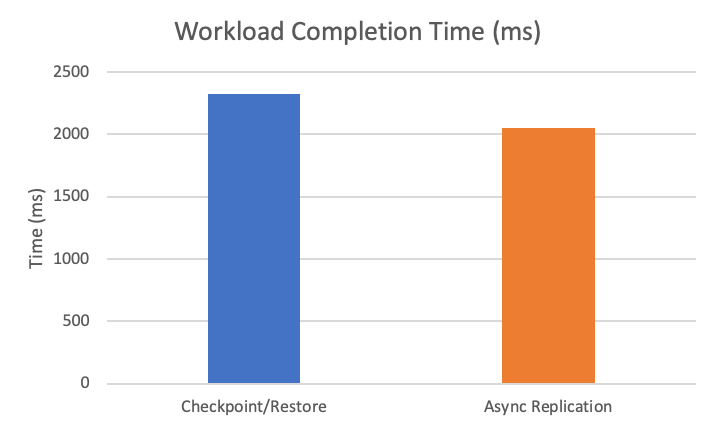
\includegraphics[scale=0.3]{../paper/async-replication}

  \hspace{1cm}

  Requests are blocked while snapshots happen, leading to slightly higher completion times.
\end{frame}

\begin{frame}{Evaluation}
  \framesubtitle{Replication Performance vs Asynchronous Replication}

  \begin{columns}
    \column{0.5\textwidth}
    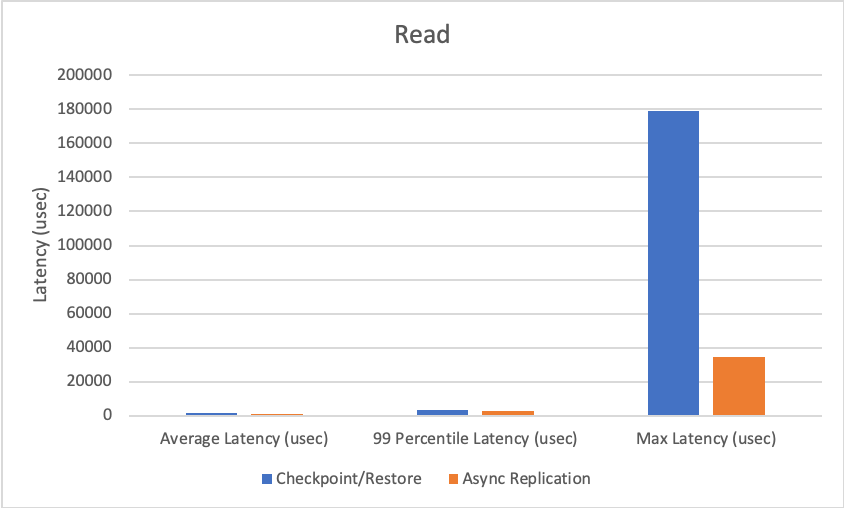
\includegraphics[scale=0.175]{../paper/async-replication-read}

    \column{0.5\textwidth}
    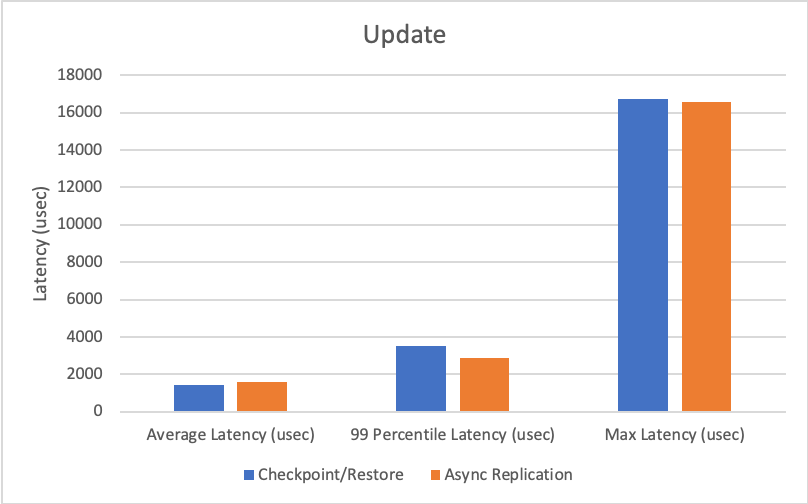
\includegraphics[scale=0.35]{../paper/async-replication-update}
  \end{columns}

  \hspace{1cm}

  \centering
  Discrepancy exists for max latency on reads due to snapshots blocking unlucky read requests.
\end{frame}

\begin{frame}{Evaluation}
  \framesubtitle{Impact of Checkpoint Frequency on
  Workload Completion}

  \centering
  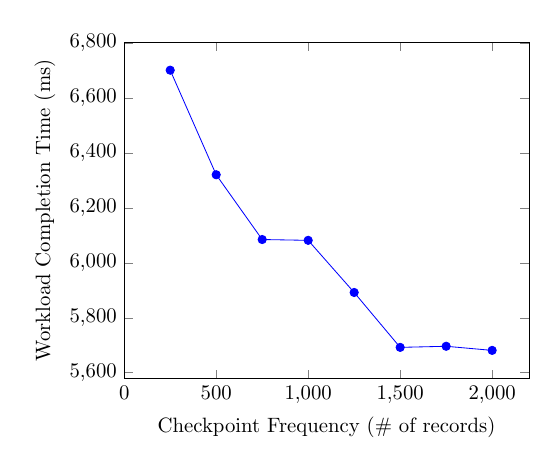
\begin{tikzpicture}[scale=0.75]
    \begin{axis}[
    xlabel=Checkpoint Frequency (\# of records),
    ylabel=Workload Completion Time (ms),
    xmin=0, xmax=2200,
    ]
    \addplot[mark=*,blue] plot coordinates {

    (250,6702)
    (500,6321)
    (750,6085)
    (1000,6082)
    (1250,5892)
    (1500,5692)
    (1750,5696)
    (2000,5681)

    };
  \end{axis}
  \end{tikzpicture}

  \hspace{1cm}

  Custom workload with 5000 insert operations with varying checkpoint intervals.
\end{frame}

\begin{frame}{Evaluation}
  \framesubtitle{Standalone vs Iterative Snapshots}

  \centering
  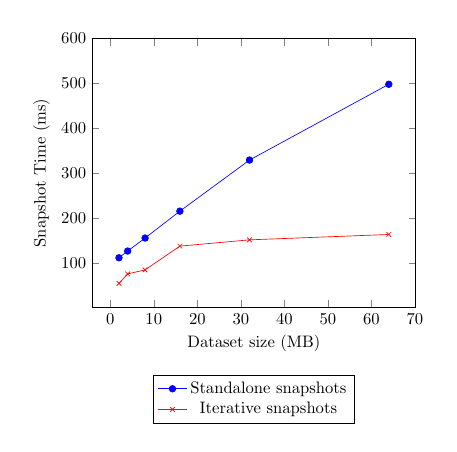
\begin{tikzpicture}[scale=0.6]
    \begin{axis}[legend style={at={(0.5,-0.25)},anchor=north},
    xlabel=Dataset size (MB),
    ylabel=Snapshot Time (ms),
    ymin=0, ymax=600, ytick={100,200,300,400,500,600}]

    \addlegendentry{Standalone snapshots}
    \addplot[mark=*,blue] plot coordinates {
    (2,111)
    (4,126)
    (8,155)
    (16,215)
    (32,329)
    (64,498)
    };

    \addlegendentry{Iterative snapshots}
    \addplot[color=red,mark=x]
    plot coordinates {
    (2,54)
    (4,75)
    (8,84)
    (16,137)
    (32,151)
    (64,163)
    };
    \end{axis}
  \end{tikzpicture}

  \hspace{1cm}

  Iterative snapshots track changes in memory pages across consecutive
  checkpoints, making it more efficient.
\end{frame}

\begin{frame}{Demo}

\end{frame}

\begin{frame}{}
  \centering \Large
  Questions?
\end{frame}

\end{document}
